% !TeX program = pdflatex
\documentclass[border=6pt]{standalone}
\usepackage{tikz}
\usetikzlibrary{arrows.meta, positioning, shapes.geometric}

\definecolor{MediumRed}{rgb}{0.925, 0.345, 0.345}
\definecolor{MediumGreen}{rgb}{0.37, 0.7, 0.66}
\definecolor{MediumBlue}{rgb}{0.015, 0.315, 0.45}
\definecolor{DarkBlue}{rgb}{0.05, 0.15, 0.35}

\begin{document}
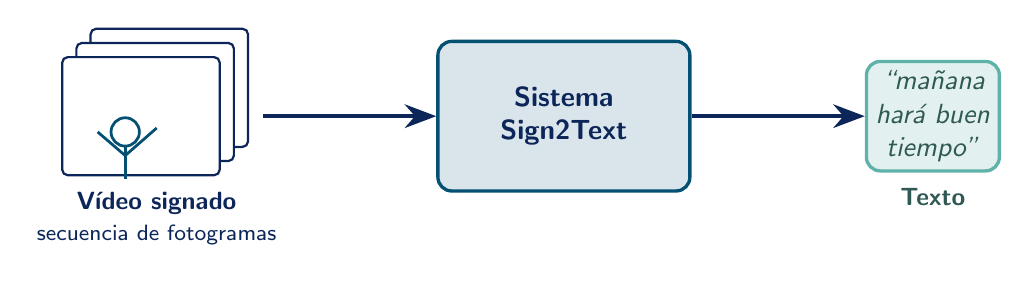
\begin{tikzpicture}[
    font=\sffamily,
    flow/.style={-{Stealth[length=4mm]}, line width=1.4pt, DarkBlue},
]

% --- vídeo de entrada: pila de fotogramas ---
\begin{scope}[shift={(0,0)}]
    \foreach \i in {2,1,0}{
        \fill[white, draw=DarkBlue, thick, rounded corners=2pt]
            (\i*0.18, \i*0.18) rectangle ++(2.0,1.5);
    }
    % iconito de "seña" en el fotograma frontal
    \draw[MediumBlue, line width=1pt] (0.8,0.55) circle (0.18);           % cabeza
    \draw[MediumBlue, line width=1pt] (0.8,0.37) -- (0.8,-0.05);          % tronco
    \draw[MediumBlue, line width=1pt] (0.8,0.25) -- (0.45,0.55);          % brazo
    \draw[MediumBlue, line width=1pt] (0.8,0.25) -- (1.2,0.6);            % brazo
\end{scope}
\node[align=center, font=\sffamily\small, text=DarkBlue] at (1.2,-0.55)
    {\textbf{Vídeo signado}\\\footnotesize secuencia de fotogramas};
\coordinate (vidout) at (2.55,0.75);

% --- sistema ---
\node[draw=MediumBlue, very thick, rounded corners=5pt, fill=MediumBlue!15,
      minimum width=3.2cm, minimum height=1.9cm, align=center, text=DarkBlue,
      right=2.2cm of vidout] (sys)
    {\textbf{Sistema}\\\textbf{Sign2Text}};

% --- texto de salida ---
\node[draw=MediumGreen, very thick, rounded corners=5pt, fill=MediumGreen!18,
      align=center, text=MediumGreen!50!black, right=2.2cm of sys] (out)
    {\textit{``mañana}\\\textit{hará buen}\\\textit{tiempo''}};
\node[align=center, font=\sffamily\small, text=MediumGreen!50!black, below=2pt of out]
    {\textbf{Texto}};

\draw[flow] (2.55,0.75) -- (sys.west);
\draw[flow] (sys.east) -- (out.west);

\end{tikzpicture}
\end{document}
